\documentclass[pdftex,a4paper,twoside,11pt]{article}
\NeedsTeXFormat{LaTeX2e}

%% Include layout, additional commands and abbreviations
%%
%% Layout definitions
%%

\usepackage[english]{babel}
\usepackage[T1]{fontenc}
\usepackage[scaled=0.91]{helvet}
\usepackage{sfmath}
\usepackage{amsmath}
\usepackage{fancyhdr}
\usepackage{fancyvrb}
\usepackage[small,bf]{caption}
\usepackage{lastpage}
\usepackage{multirow}
\usepackage{tabularx}
\usepackage{longtable}
\usepackage{graphicx}
\usepackage{url}
\usepackage[usenames,dvipsnames]{color}

\definecolor{darkblue}{rgb}{0,0,0.5}
\definecolor{red}{rgb}{1,0,0}
\definecolor{green}{rgb}{0,1,0}
\definecolor{orange}{rgb}{1,0.5,0}

\usepackage[pdftex,
            colorlinks=true,
            pdfstartview=FitV,
            linkcolor=darkblue,
            citecolor=darkblue,
            urlcolor=blue,
            plainpages=false,
            pdfpagelabels,
            linktocpage,
            backref,
            pagebackref]{hyperref}

\hypersetup{
  pdftitle={CR2RES Reflex Tutorial},
  pdfauthor={CR2RES Pipeline Team},
  pdfkeywords={CR2RES, Data Reduction, Pipeline, Reflex, Tutorial},
  pdfsubject={CR2RES Reflex Tutorial}
}
\usepackage[public]{dmd-doc}

%%% Local Variables: 
%%% mode: latex
%%% TeX-master: t
%%% End:

%%
%% Abbreviations and extra command definitions
%%

%%
%% Release information
%%

\newcommand{\instrument}{\mbox{CRIRES{\fontfamily{pbk}\fontseries{db}\selectfont+}}}
\newcommand{\release}{0.9.4}

%%
%% Abbreviations
%%

\newcommand{\eg}{{e.g.~}}
\newcommand{\ie}{{i.e.~}}

\newcommand{\degr}{\hbox{$^\circ$}}
\newcommand{\arcmin}{\hbox{$^\prime$}}
\newcommand{\arcsec}{\hbox{$^{\prime\prime}$}}
\newcommand{\celsius}{\hbox{$^{\circ}\mathsf{C}$}}

\newcommand{\CPL}{\textit{Common Pipeline Library}\/}
\newcommand{\esorex}{\mbox{EsoRex}}
\newcommand{\gasgano}{\mbox{Gasgano}}
\newcommand{\reflex}{\textit{\mbox{Reflex}}\/}

%%
%% Additional commands
%%

\newcommand{\tbspa}{\rule[1ex]{0pt}{1.1ex}}
\newcommand{\tbspb}{\rule[-1.0ex]{0pt}{1.0ex}}
\newcommand{\tcen}{\raisebox{-7pt}[7pt][0pt]}

\newcommand{\units}[1]{\ensuremath{\:\mathsf{#1}}}

\newcommand{\figref}[1]{\figurename~\ref{#1}}
\newcommand{\tabref}[1]{\tablename~\ref{#1}}

\newcommand{\red}[1]{\color{red}{#1}\color{black}}

\newcommand{\putgraph}[4]{
    \begin{figure}[ht]
        \begin{center}
    \includegraphics[width=#1]{#2}
    \end{center}
    \caption{\it #4.}
    \label{fig:#3}
    \end{figure}
}

\newcommand{\putgraphhere}[4]{
    \begin{figure}[h!]
        \begin{center}
    \includegraphics[width=#1]{#2}
    \end{center}
    \caption{\it #4.}
    \label{fig:#3}
    \end{figure}
}




\dmdProgram{GEN}
\dmdProject{Science Operation Software Department}
\dmdTitle{Reflex CR2RES Tutorial}
\dmdDocId{ESO-XXXXXX}
\dmdDocVersion{0.9.4}
\dmdDocType{Manual (MAN)}
\dmdDocDate{2021-09-10}

\dmdPreparedBy{CR2RES Pipeline Team}
\dmdValidatedBy{}
\dmdApprovedBy{}

%% Additional commands and abbreviations
\graphicspath{{../figures/}{../pipedoc/figures/}}

%% Remember to update shortcut.tex
\def\reldate{\releasedate}
\def\pipeno{\pipelinevers}
\def\kitno{\pipeno}
\def\docno{\pipelinemanualvers}
\def\qfitsno{\qfitsvers}
\def\cplno{\cplvers}
\def\esorexno{\esorexvers}
\def\reflexno{\reflexvers}
\def\gasganono{\gasganovers}
\def\jdkno{\jdkvers}
\def\dmdissue{\docno}

\setlongtables
\makeindex
\bibliographystyle{plain} 

\begin{document}
\pagenumbering{arabic}
\dmdmaketitle
\emptypage{This page was intentionally left blank}

\section*{Authors}
\begin{tabularx}{\linewidth}{|p{0.25\linewidth}|X|}
  \hline
  \multicolumn{1}{|l|}{\textbf{Name}}\tbspa &
  \multicolumn{1}{l|}{\textbf{Affiliation}} \tbspb \\
  \hline
  \tbspa
  N.N. & Far out in the uncharted backwaters of the unfashionable end of the western spiral arm of the Galaxy
  \tbspb\\
  \hline
\end{tabularx}
\emptypage{This page was intentionally left blank}

\section*{Change Record from previous Version}
\begin{tabularx}{\linewidth}{|p{0.25\linewidth}|X|}
  \hline
  \multicolumn{1}{|l|}{\textbf{Affected Section(s)}}\tbspa &
  \multicolumn{1}{l|}{\textbf{Changes/Reason/Remarks}}\tbspb \\
  \hline
  \tbspa
  All                      & First draft
  \tbspb\\
  \hline
\end{tabularx}
\emptypage{This page was intentionally left blank}

\tableofcontents
\cleardoublepage

\section{Introduction And Scope}

{\tt Reflex}\footnote{User support for this software is available by sending 
enquiries to \mail{usd-help@eso.org}} is the ESO Recipe Flexible Execution 
Workbench, an environment to run ESO VLT pipelines which employs a workflow 
engine (Kepler\footnote{\http{kepler-project.org}}) to provide a real-time
visual representation of a data reduction cascade, called a workflow,
which can be easily understood by most astronomers.  This document is
a tutorial designed to enable the user to employ the \instname\, workflow to
reduce his/her data in a user-friendly way, concentrating on
high-level issues such as data reduction quality and signal-to-noise 
(S/N) optimisation.

A workflow accepts science and calibration data, as delivered to PIs
in the form of PI-Packs (until October 2011) or downloaded from the
archive using the CalSelector
tool\footnote{\http{www.eso.org/sci/archive/calselectorInfo.html}} and
organises them into DataSets, where each DataSet contains one
science object observation (possibly consisting of several science
files) and all associated raw and static calibrations required for a
successful data reduction. The data organisation process is fully
automatic, which is a major time-saving feature provided by the
software. The DataSets selected by the user for reduction are fed
through the workflow which executes the relevant pipeline recipes (or
stages) in the correct order.
%, providing optional user interactivity at
%key data reduction points with the aim of enabling the iteration of
%certain recipes in order to obtain better results. 
Full control of the
various recipe parameters is available within the workflow, and the
workflow deals automatically with optional recipe inputs via built-in
conditional branches. Additionally, the workflow stores the reduced
final data products in a logically organised directory structure and
employing user-configurable file names.
 %This file is in the pipedoc directory

Add here some explanation about this specific workflow. Instrument modes supported, etc...

\section{Software Installation}

The software pre-requisites for {\tt Reflex \reflexvers} may be found at:\newline
  \http{www.eso.org/sci/software/pipelines/reflex\_workflows}

To install the {\tt Reflex \reflexvers} software and demo data, 
please follow these instructions:
\begin{enumerate}
  \item From any directory, download the installation script:
        {\small
        \begin{verbatim}
        wget ftp://ftp.eso.org/pub/dfs/reflex/install_reflex
        \end{verbatim}
        }

  \item Make the installation script executable:
        {\small
        \begin{verbatim}
        chmod u+x install_reflex
        \end{verbatim}
        }

  \item Execute the installation script:
        {\small
        \begin{verbatim}
        ./install_reflex
        \end{verbatim}
        }
        and the script will ask you to specify three directories: the download
        directory {\tt \verb|<|download\_dir\verb|>|}, the software
        installation directory {\tt \verb|<|install\_dir\verb|>|}, 
        and the directory to be used to store the demo data 
        {\tt \verb|<|data\_dir\verb|>|}.
        If you do not specify these directories, then the installation script 
        will create them in the current directory with default names.

  \item You will be given a choice of pipelines (with the corresponding 
        workflows) to install. Please specify the numbers for the pipelines 
        you require, separated by a space, or type ``A'' for all pipelines.

  \item To start {\tt Reflex}, issue the command:
        {\small
        \begin{verbatim}
        <install_dir>/bin/reflex
        \end{verbatim}
        }
        It may also be desirable to set up an alias command for starting the 
        {\tt Reflex} software, using the shell command {\tt alias}. 
        Alternatively, the {\tt PATH} variable can be updated to contain the
        {\tt \verb|<|install\_dir\verb|>|/bin} directory.
\end{enumerate}
 %This file is in the pipedoc directory

\section{Demo Data}
Add some explanation about the demo data used.

\section{Quick Start: Reducing The Demo Data \label{sec:quick_start}}

Add here a two pages maximum explanation on how to quickly reduce the demo data set.

\section{About The Reflex Canvas \label{sec:about_canvas}}

\subsection{Saving And Loading Workflows}

In the course of your data reductions, it is likely that you will
customise the workflow for various data sets, even if this simply consists of 
editing the {\tt ROOT\_DATA\_DIR} to a different value for each data set. 
Whenever you modify a workflow in any way, you have the option of saving the 
modified version to an {\tt XML} file using {\tt File -> Export As} 
(which will also open a new workflow canvas corresponding to the saved file). 
The saved workflow may be opened in subsequent
{\tt Reflex} sessions using {\tt File -> Open}. Saving the workflow in the
default format (.kar) is only advised if you do not plan to use the workflow
in other computer.

\subsection{Buttons}  
         
At the top of the {\tt Reflex} canvas are a set of buttons which have the following useful functions:
\begin{itemize}
\item{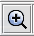
\includegraphics[width=0.5cm,height=0.5cm]{reflex_zoom_in_button.png} - Zoom in.}
\item{
\includegraphics[width=0.5cm,height=0.5cm]{reflex_zoom_reset_button.png} - Reset the zoom to 100\%.}
\item{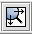
\includegraphics[width=0.5cm,height=0.5cm]{reflex_zoom_to_fit_button.png} - Zoom the workflow to fit the current window size (Recommended).}
\item{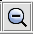
\includegraphics[width=0.5cm,height=0.5cm]{reflex_zoom_out_button.png} - Zoom out.}
\item{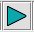
\includegraphics[width=0.5cm,height=0.5cm]{reflex_run_button.png} - Run (or resume) the workflow.}
\item{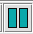
\includegraphics[width=0.5cm,height=0.5cm]{reflex_pause_button.png} - Pause the workflow execution.}
\item{
\includegraphics[width=0.5cm,height=0.5cm]{reflex_stop_button.png} - Stop the workflow execution.}
\end{itemize}
The remainder of the buttons (not shown here) are not relevant to the 
workflow execution.

\subsection{Workflow States}

A workflow may only be in one of three states: executing, paused, or stopped.
 These states are indicated by the yellow highlighting of the
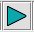
\includegraphics[width=0.5cm,height=0.5cm]{reflex_run_button.png},
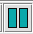
\includegraphics[width=0.5cm,height=0.5cm]{reflex_pause_button.png},
and 
\includegraphics[width=0.5cm,height=0.5cm]{reflex_stop_button.png}
buttons, respectively. A workflow is executed by clicking the
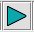
\includegraphics[width=0.5cm,height=0.5cm]{reflex_run_button.png} button. 
Subsequently the workflow and any running
pipeline recipe may be stopped immediately by clicking the

\includegraphics[width=0.5cm,height=0.5cm]{reflex_stop_button.png}
button, or the workflow may be paused by clicking the 
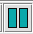
\includegraphics[width=0.5cm,height=0.5cm]{reflex_pause_button.png} button which
will allow the current actor/recipe to finish execution before the workflow is 
actually paused. Note that after clicking the
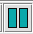
\includegraphics[width=0.5cm,height=0.5cm]{reflex_pause_button.png} button, 
it is possible that more than one actor is executed, since this behaviour 
depends on the workflow scheduling. For instance, if there are two actors in 
parallel, and you pause the workflow while one is being executed, then both
of them will be executed before the workflow is actually paused. After pausing,
the workflow may be resumed by clicking the
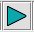
\includegraphics[width=0.5cm,height=0.5cm]{reflex_run_button.png} button again.

\subsection{The Runtime Window}

You may find the runtime window a useful aid in monitoring the
reduction progress of your data. This window may be started by
clicking {\tt Workflow -> Runtime Window} from the {\tt Reflex} canvas
menu. You will notice that on the left-hand side the runtime window
has buttons allowing the control of the workflow (\fbox{\tt Go},
\fbox{\tt Pause}, \fbox{\tt Resume}, \fbox{\tt Stop}) and text boxes
for controlling workflow parameters such as the working data directory
etc.

On the right-hand side of the runtime window is a text box with the
title ``Recipe Status'' which lists the current status of each
pipeline recipe and the reduction status of each DataSet. A recipe may
have the following status values:
\begin{itemize}
\item{{\tt Not Running} - The recipe has not yet been run for any DataSet so far.}
\item{{\tt Executing} - The recipe is currently executing for a DataSet.}
\item{{\tt Done} - The last execution of the pipeline recipe was successful.}
\item{{\tt Failed} - The recipe failed on the last DataSet.}
\item{{\tt Skip} - The recipe was skipped for the last DataSet.}
\item{{\tt Disabled} - The recipe was disabled for the last DataSet.}
\item{{\tt Stopped} - The workflow was stopped during the reduction of a DataSet.}
\end{itemize}

Below the list of recipe status values is a detailed list of input and
output files used for each DataSet within each recipe execution. This
information is sometimes very useful for the user who wants to know
exactly which files were used as input for a particular DataSet for a
given pipeline recipe, and where the relevant output files were
written.
 %This file is in the pipedoc directory
\section{The \instname\, Workflow \label{sec:wkf_general_desc}}

The \instname\,  workflow canvas is organised into a number of areas.
From top-left to top-right you
will find general workflow instructions, directory parameters, and
global parameters.  In the middle row you will find five boxes
describing the workflow general processing steps in order from left to
right, and below this the workflow actors themselves are organised
following the workflow general steps. 

\subsection{Workflow Canvas Parameters \label{sec:wkf_canvpar}}

The workflow canvas displays a number of parameters that may be set by
the user. Under ``Setup
Directories'' the user is only required to set the {\tt
  ROOT\_DATA\_DIR} to the working directory for the DataSet(s) to be
reduced, which, by default, is set to the directory containing the
demo data. Raw data should be stored in a subdirectory of {\tt
  ROOT\_DATA\_DIR}, defined by the parameter {\tt RAWDATA\_DIR}, which
is recursively scanned by the {\tt Data Organiser} actor for input raw
data. The directory {\tt CALIB\_DATA\_DIR}, which is within the
pipeline installation directory, is also scanned by the {\tt Data
  Organiser} actor to find any static calibrations that may be missing
in your DataSet(s).  If required, the user may edit the directories
{\tt BOOKKEEPING\_DIR}, {\tt LOGS\_DIR}, {\tt TMP\_PRODUCTS\_DIR}, and
{\tt END\_PRODUCTS\_DIR}, which correspond to the directories where
book-keeping files, logs, temporary products and end products are
stored, respectively (see the Reflex User Manual for further details;
\cite{REFLEXMAN}).

Under the ``Global Parameters'' area of the workflow canvas, the user
may set the {\tt FITS\_VIEWER} parameter to the command used for
running his/her favourite application for inspecting FITS
files. Currently this is set by default to {\tt fv}, but other
applications, such as {\tt ds9}, {\tt skycat} and {\tt gaia} for
example, may be useful for inspecting image data.

By default the {\tt EraseDirs} parameter is set to {\tt false}, which
means that no directories are cleaned before executing the workflow,
and the recipe actors will work in Lazy mode (see
Section~\ref{sec:lazy_mode}), reusing the previous pipeline recipe outputs
where input files and parameters are the same as for the previous
execution, which saves considerable processing time. Sometimes it is
desirable to set the {\tt EraseDirs} parameter to {\tt true}, which
forces the workflow to recursively delete the contents of the
directories specified by {\tt BOOKKEEPING\_DIR}, {\tt LOGS\_DIR}, and
{\tt TMP\_PRODUCTS\_DIR}. This is useful for keeping disk space usage
to a minimum and will force the workflow to fully rereduce the data
each time the workflow is run.


 %This file is in the pipedoc directory
\subsection{Workflow Actors}
\subsubsection{Simple Actors \label{sec:simple_actors}}

Simple actors have workflow symbols that consist of a single (rather than multiple) green-blue rectangle. They may also have a logo within the rectangle
to aid in their identification. The following actors are simple actors:
\begin{itemize}
\item{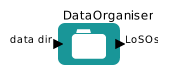
\includegraphics[width=2.5cm,height=1.3cm]{reflex_data_organiser_actor.png} - The {\tt Data Organiser} actor.}
\item{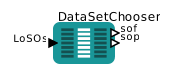
\includegraphics[width=2.5cm,height=1.6cm]{reflex_data_set_chooser_actor.png} - The {\tt Data Set Chooser} actor.}
\item{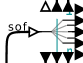
\includegraphics[width=1.6cm,height=0.8cm]{reflex_fits_router_actor.png} - The {\tt Fits Router} actor}
\item{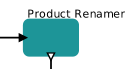
\includegraphics[width=1.8cm,height=1cm]{reflex_product_renamer_actor.png} - The {\tt Product Renamer} actor.}
\item{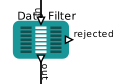
\includegraphics[width=2.2cm,height=1cm]{reflex_data_filter_actor.png} - The {\tt Data Filter} actor.}
\end{itemize}

Access to the parameters for a simple actor is achieved by
right-clicking on the actor and selecting {\tt Configure Actor}. This
will open an ``Edit parameters'' window. Note that the {\tt Product Renamer}
actor is a jython script (Java implementation of the Python
interpreter) meant to be customised by the user (by double-clicking on
it).

 %This file is in the pipedoc directory

Add here a description of this workflow specific actors 
(probably including some composite actors).

\subsubsection{Lazy Mode \label{sec:lazy_mode}}

By default, all recipe executer actors in a pipeline workflow are
``Lazy Mode'' enabled. This means that when the workflow attempts to
execute such an actor, the actor will check whether the relevant
pipeline recipe has already been executed with the same input files
and with the same recipe parameters. If this is the case, then the
actor will not execute the pipeline recipe, and instead it will simply
broadcast the previously generated products to the output port. The
purpose of the Lazy mode is therefore to minimise any reprocessing of
data by avoiding data rereduction where it is not necessary.
  
One should note that the actor Lazy mode depends on the contents of
the directory specified by \\ {\tt BOOKKEEPING\_DIR} and the relevant
FITS file checksums. Any modification to the directory contents and/or
the file checksums will cause the corresponding actor when executed to
run the pipeline recipe again, thereby rereducing the input data.

The forced rereduction of data at each execution may of course be
desirable. To force a rereduction of all data for all {\tt RecipeExecuter}
actors in the workflow (i.e. to disable Lazy mode for the whole
workflow), set the {\tt EraseDirs} parameter under the ``Global
Parameters'' area of the workflow canvas to {\tt true}. This will then
remove all previous results as well.  To force a rereduction of data
for any single  {\tt RecipeExecuter} actor in the workflow (which will be
inside the relevant composite actor), right-click the  {\tt RecipeExecuter} actor, select
{\tt Configure Actor}, and uncheck the Lazy mode parameter tick-box in
the ``Edit parameters'' window that is displayed.

 %This file is in the pipedoc directory

Add here a description of the workflow steps like Data organisation,
routing, creation of calibration files and science reduction.

Add here a description on how to optimise the results of the workflow.

\section{Frequently Asked Questions}

\begin{itemize}
   \item {\bf Where are my intermediate pipeline products?}
   Intermediate pipeline products are stored in the directory {\tt
   \verb|<|TMP\_PRODUCTS\_DIR\verb|>|} (defined on the workflow canvas)
   and organised further in directories by pipeline recipe.

%\item {\bf I have many DataSets in my data directory. How can I reduce
%  them interactively without having to wait a long time between
%  interactive windows being displayed?}

%Reduce all the DataSets at once with the interactive windows disabled
%for all interactive actors. When this reduction has finished, you
%should re-enable the interactive windows that you require, and run the
%workflow again. The workflow will run in Lazy mode and no time will be
%spent on pipeline reductions, unless you specifically change a
%parameter in one of the interactive windows.
        
%      Note that Lazy mode will not work if the workflow parameter {\tt
%        EraseDirs} is set to {\tt true}.

   \item {\bf Can I use different sets of bias frames to calibrate my
          flat frames and science data?}
   Yes. In fact this is what is currently implemented in the workflow(s).
   Each file in a DataSet has a purpose attached to it (\cite{REFLEXMAN}).
   It is this purpose that is used by the workflow to send the correct
   set of bias frames to the recipes for flat frame combination and 
   science frame reduction, which may or may not be the same set of bias 
   frames in each case.

   \item {\bf Can I launch {\tt Reflex} from the command line?}
   Yes, use the command:
      \begin{verbatim}
      reflex -- -runwf -nocache -nogui <workflow_path>/<workflow>.xml
      \end{verbatim}
   Note that this mode is not fully supported, and the user should be 
   aware of two points. Firstly, the execution prompt is not returned after the
   workflow finishes, and therefore {\tt Reflex} must be manually killed.
   Secondly, all the interactive windows will still appear (if activated in the
   workflow), so it is not suitable for batch processing.
        
   \item {\bf How can I add new actors to an existing workflow?}
   You can drag and drop the actors in the menu on the left of the {\tt Reflex} 
   canvas. Under {\tt Eso-reflex -> Workflow} you may find all the actors
   relevant for pipeline workflows, with the exception of the recipe executer.
   This actor must be manually instantiated using
   {\tt Tools -> Instantiate Component}. Fill in the ``Class name'' field with 
   {\tt org.eso.RecipeExecuter} and in the pop-up window choose the required 
   recipe from the pull-down menu. To connect the ports of the actor, click on
   the source port, holding down the left mouse button, and release the mouse
   button over the destination port. Please consult the Reflex User Manual
   (\cite{REFLEXMAN}) for more information.

   \item {\bf How can I broadcast a result to different subsequent actors?}
   If the output port is a multi-port (filled in white), then you may have
   several relations from the port. However, if the port is a single port
   (filled in black), then you may use the black diamond from the toolbar.
   Make a relation from the output port to the diamond. Then make relations 
   from the input ports to the diamond. Please note that you cannot click to 
   start a relation from the diamond itself. Please consult the Reflex User 
   Manual (\cite{REFLEXMAN}) for more information.

   \item {\bf How can I run manually the recipes executed by Reflex?}
   If a user wants to re-run a recipe on the command line he/she has to go to
   the appropriate reflex\_book\_keeping directory, which is generally 
   reflex\_book\_keeping/\instname/<recipe\_name>\_<number> (for instance 
   reflex\_book\_keeping/\instname/bias\_1/). There, subdirectories exist with 
   the time stamp of the recipe execution (e.g. 2013-01-25T12:33:53.926/). 
   If the user wants to re-execute the most recent processing he/she should 
   go to the {\tt latest} directory and then execute 
   {\tt ESOREX\_CONFIG="REFLEX\_INST/etc/esorex.rc 
   REFLEX\_INST/bin/esorex --recipe-config=<recipe>.rc <recipe> data.sof}, 
   where REFLEX\_INST is the directory where Reflex and the pipelines were
   installed. If the user knows the name of the input raw files for the 
   recipe, the correct directory among the many time stamps can be found via 
   {\tt grep <raw\_file> */data.sof}. Afterwards the procedure is the same 
   as before. The products will appear in the directory from which the recipe
   is called, and not in the reflex\_tmp\_products or reflex\_end\_products
   directory, and they will not be renamed. 

\end{itemize}


Add here a section on troubleshooting problems.

%\bibliography{cr2res_reflex_tutorial}
\end{document}
